\chapter{Nevronske mreže}

V tem poglavju bomo podrobneje predstavili naprej usmerjene (angl.\ feedforward) umetne nevronske mreže, natančneje večnivojske perceptrone (angl.\ multilayer perceptron). Zaradi boljše berljivosti bomo v nadaljevanju uporabljali zgolj izraz nevronska mreža. Najprej bomo predstavili osnovne koncepte, nato podali matematični model ter opisali algoritem vzvratnega razširjanja napake.

%%%%%%%%%%%%%%%%%%%%%%%%%%%%%%%%%%%%%%%%%%%%%%%%%%%%%%%%%%%%%%%%%%%%%%%%%%%%%%%%%%%%%%%%%%%%%

\section{Osnovni koncepti}

Umetna nevronska mreža je matematični model, ki posnema delovanje človeških možganov. Predstavljamo si jo lahko kot usmerjen acikličen graf, kjer so vozlišča oziroma nevroni urejeni v zaporedne sloje. Povezave med njimi so utežene in potekajo izključno med nevroni sosednjih slojev, v smeri od prvega (vhodnega) sloja proti zadnjemu (izhodnemu) sloju. Sloje običajno razdelimo na tri tipe:
\begin{itemize}
  \item \textbf{Vhodni sloj} je prvi sloj, ki sprejme vhodne podatke in jih brez sprememb posreduje skritemu sloju. Število nevronov v tem sloju ustreza dimenziji vhodne množice.
  \item \textbf{Skriti sloji} se nahajajo med vhodnim in izhodnim slojem ter so odgovorni za večino obdelave podatkov. Njihovo število in velikost se lahko poljubno prilagajata glede na kompleksnost problema.
  \item \textbf{Izhodni sloj} je zadnji sloj in vrne končni rezultat, ki predstavlja napoved mreže. Število nevronov v tem sloju je odvisno od vrste problema – pri regresiji je to običajno en nevron, pri klasifikaciji pa en nevron za vsak razred. 
\end{itemize}

\begin{figure}[H]
  \centering
  % LAYERS IN NEURAL NETWORK
\begin{tikzpicture}[scale=1.25,x=2.2cm,y=1.4cm]

  \message{^^Layers in Neural network}
  \readlist\Nnod{4,5,5,5,3} % array of number of nodes per layer
  \readlist\Nstr{n,m,m,m,k} % array of string number of nodes per layer
  % \readlist\Cstr{\strut x,a^{(\prev)},a^{(\prev)},a^{(\prev)},y} % array of coefficient symbol per layer
  \def\yshift{0.5} % shift last node for dots
  
  \message{^^Drawing Layers}
  \foreachitem \N \in \Nnod{ % loop over layers
    \def\lay{\Ncnt} % alias of index of current layer
    \pgfmathsetmacro\prev{int(\Ncnt-1)} % number of previous layer
    \message{\lay,}
    \foreach \i [evaluate={\c=int(\i==\N); \y=\N/2-\i-\c*\yshift;
                 \index=(\i<\N?int(\i):"\Nstr[\lay]");
                 \x=\lay; \n=\nstyle;}] in {1,...,\N}{ % loop over nodes
      % NODES
      \node[node \n] (N\lay-\i) at (\x,\y) {}; % {$\Cstr[\lay]_{\index}$};
      
      % CONNECTIONS
      \ifnum\lay>1 % connect to previous layer
        \foreach \j in {1,...,\Nnod[\prev]}{ % loop over nodes in previous layer
          \draw[connect arrow, gray] (N\prev-\j) -- (N\lay-\i); % connect arrows directly
        }
      \fi % else: nothing to connect first layer
      
    }
    \path (N\lay-\N) --++ (0,1+\yshift) node[midway,scale=1.5] {$\vdots$};
  }
  
  % RECTANGLE
  \node[
    draw=myblue!40,
    fill=myblue,
    fill opacity=0.02,
    rounded corners=2,
    inner sep=10pt,
    fit=(N2-1)(N4-5)
  ] {};

  % LABELS
  \node[above=5,align=center,softorange!60!black] at (N1-1.90) {vhodni\\[-0.2em]sloj};
  \node[above=10,align=center,myblue!60!black] at (N3-1.90) {skriti sloji};
  \node[above=5,align=center,myred!60!black] at (N\Nnodlen-1.90) {izhodni\\[-0.2em]sloj};
  
\end{tikzpicture}

  \caption{Sloji v nevronski mreži}~\label{fig:nn-layers}
\end{figure}

Izhodno vrednost nevrona imenujemo aktivacija. Vsak nevron sprejme aktivacije nevronov iz prejšnjega sloja, oziroma vhodne podatke v primeru prvega sloja. Iz teh vrednosti izračuna uteženo vsoto, nato pa rezultat preslika s t.\  i.\ aktivacijsko funkcijo. Aktivacijska funkcija je praviloma nelinearna, kar zagotavlja nelinearnost modela.
Da bi utežena vsota lahko vsebovala konstantni člen, vsakemu sloju razen izhodnega dodamo po en nevron s konstantno aktivacijo ena.

\begin{figure}[H]
  \centering
  \tikzset{
  connect arrow/.style={->, draw=gray}
}

% LAYERS IN NEURAL NETWORK
\begin{tikzpicture}[scale=1.25,x=2.2cm,y=1.4cm]

  \message{^^Layers in Neural network}
  \readlist\Nnod{4,5,5,5,3} % array of number of nodes per layer
  \readlist\Nstr{n,m,m,m,k} % array of string number of nodes per layer
  % \readlist\Cstr{\strut x,a^{(\prev)},a^{(\prev)},a^{(\prev)},y} % array of coefficient symbol per layer
  \def\yshift{0.5} % shift last node for dots
  
  \message{^^Drawing Layers}
  \foreachitem \N \in \Nnod { % loop over layers
    \def\lay{\Ncnt} % current layer index
    \pgfmathsetmacro\prev{int(\Ncnt - 1)} % previous layer index
    \message{\lay,}

    % Number of total nodes in this layer including bias if not last
    \ifnum\lay<\Nnodlen
      \pgfmathsetmacro\Nwithbias{\N + 1}
      \def\firstIndex{0}
    \else
      \pgfmathsetmacro\Nwithbias{\N}
      \def\firstIndex{1}
    \fi

    % All neurons in layer: bias (index 0) + regular (1..N)
    \foreach \i [evaluate={
        \c=int(\i==\N);
        \y=\N/2-\i-\c*\yshift;
        \x=\lay; \n=\nstyle;
      }] in {\firstIndex,...,\N} {

      % \node[node \n] (N\lay-\i) at (\x,\y) {};

      \ifnum\i=0
        % \node[circle, draw=teal!60!black, fill=teal!20, minimum size=8pt, inner sep=2pt] (N\lay-\i) at (\x,\y) {};
        \node[node bias] (N\lay-\i) at (\x,\y) {+1};
      \else
        \node[node \n] (N\lay-\i) at (\x,\y) {};
      \fi

      % Only connect if NOT bias node
      \ifnum\i>0
        \ifnum\lay>1
          \ifnum\prev<\Nnodlen
            \foreach \j in {0,...,\Nnod[\prev]} {
              \draw[connect arrow] (N\prev-\j) -- (N\lay-\i);
            }
          \else
            \foreach \j in {1,...,\Nnod[\prev]} {
              \draw[connect arrow] (N\prev-\j) -- (N\lay-\i);
            }
          \fi
        \fi
      \fi
    }

    % Dots
    \path (N\lay-\N) --++ (0,1+\yshift) node[midway,scale=1.5] {$\vdots$};
  }
  
  % RECTANGLE
  % \node[
  %   draw=myblue!40,
  %   fill=myblue,
  %   fill opacity=0.02,
  %   rounded corners=2,
  %   inner sep=10pt,
  %   fit=(N2-1)(N4-5)
  % ] {};

  % LABELS
  % \node[above=5,align=center,softorange!60!black] at (N1-1.90) {vhodni\\[-0.2em]sloj};
  % \node[above=10,align=center,myblue!60!black] at (N3-1.90) {skriti sloji};
  % \node[above=5,align=center,myred!60!black] at (N\Nnodlen-1.90) {izhodni\\[-0.2em]sloj};
  
\end{tikzpicture}

  \caption{Nevron s konstantno aktivacijo}~\label{fig:nn-bias}
\end{figure}

%%%%%%%%%%%%%%%%%%%%%%%%%%%%%%%%%%%%%%%%%%%%%%%%%%%%%%%%%%%%%%%%%%%%%%%%%%%%%%%%%%%%%%%%%%%%%

\section{Matematični model}

V nadaljevanju bomo definirali notacijo, ki je pogosto uporabljena v strokovni literaturi s področja umetne inteligence, na primer v~\cite{Hastie2009}. Takšna notacija omogoča dosledno in formalno predstavitev nevronskih mrež.

Naj bo nevronska mreža sestavljena iz $k+1$ slojev, označenih z $L^{(0)}, L^{(1)}, \dots, L^{(k)}$, kjer je $L^{(0)}$ vhodni sloj, $L^{(k)}$ pa izhodni sloj. Vsak sloj $L^{(i)}$ vsebuje $N^{(i)}$ nevronov, za $i = 0, \dots, k$.

Vhod v mrežo predstavimo z vektorjem $x \in \mathbb{R}^{N^{(0)}}$, ki vsebuje $N^{(0)}$ komponent in služi kot začetna aktivacija v vhodnem sloju.

Za sloje nevronske mreže uvedemo naslednje pojme:

\begin{itemize}
  \item $a^{(i)}$ aktivacijska funkcija v sloju $L^{(i)}$, za $i = 1, \dots, k$.
  
  \item $h^{(i)} = \left(h^{(i)}_1, h^{(i)}_2, \dots, h^{(i)}_{N^{(i)}}\right)$ je vektor aktivacij v sloju $L^{(i)}$, za $i = 0, \dots, k$. Za vhodni sloj velja $h^{(0)} = x$.
  
  \item $z^{(i)} = \left(z^{(i)}_1, z^{(i)}_2, \dots, z^{(i)}_{N^{(i)}}\right)$ je vektor uteženih vsot v sloju $L^{(i)}$, za $i = 1, \dots, k$, pri čemer vsaka komponenta predstavlja vsoto uteženih vhodov za posamezen nevron:
  \[
    z^{(i)}_j = \sum_{\ell=1}^{N^{(i-1)}} w^{(i)}_{j\ell} h^{(i-1)}_\ell + b^{(i)}_j, \quad \text{za } j = 1, \dots, N^{(i)}.
  \]

  \item $W^{(i)}$ je matrika uteži dimenzije $N^{(i)} \times N^{(i-1)}$, ki povezuje sloj $L^{(i-1)}$ s slojem $L^{(i)}$, za $i = 1, \dots, k$. Ima naslednjo obliko:
  \[
    W^{(i)} = \begin{bmatrix}
      w^{(i)}_{1,1} & w^{(i)}_{1,2} & \cdots & w^{(i)}_{1,N^{(i-1)}} \\
      w^{(i)}_{2,1} & w^{(i)}_{2,2} & \cdots & w^{(i)}_{2,N^{(i-1)}} \\
      \vdots       & \vdots       & \ddots & \vdots               \\
      w^{(i)}_{N^{(i)},1} & w^{(i)}_{N^{(i)},2} & \cdots & w^{(i)}_{N^{(i)},N^{(i-1)}}
    \end{bmatrix}
  \]

  \item $b^{(i)} = \left(b^{(i)}_1, b^{(i)}_2, \dots, b^{(i)}_{N^{(i)}}\right)$ je vektor uteži nevronov s konstantno aktivacijo (angl.\ bias) za sloj $L^{(i)}$, za $i = 1, \dots, k$.
\end{itemize}

Aktivacije v sloju $L^{(i)}$ izračunamo s pomočjo aktivacijske funkcije $a^{(i)}$, ki se uporablja po komponentah:
  \[
    h^{(i)}_j = a^{(i)}\left(z^{(i)}_j\right), \quad \text{za } j = 1, \dots, N^{(i)}.
  \]

Postopek se iterativno izvede za sloje $i = 1, \dots, k$, pri čemer vektor $h^{(k)}$ predstavlja izhod mreže.

TODO:

Povratno razširjanje (angl.~\textit{backpropagation}) je metoda za učenje v umetnih nevronskih mrežah, ki temelji na minimizaciji funkcije izgube z gradientnim spustom. Širšo pozornost je pritegnila v delu Rumelharta, Hintona in Williamsa leta 1986~\cite{rumelhart1986learning}.

Naj bo \( X \in \mathbb{R}^{N \times d} \) matrika vhodnih podatkov, kjer vsak vhodni primer \( x^{(i)} \in \mathbb{R}^d \) predstavlja vrstico, in \( y \in \mathbb{R}^{N \times c} \) matrika pripadajočih ciljev, kjer je \( c \) število razredov. Učni cilj je minimizirati povprečno funkcijo izgube:
\[
\mathcal{J}(W) = \frac{1}{N} \sum_{i=1}^N \mathcal{L}(h^{(k)}(x^{(i)}), y^{(i)}),
\]
kjer je \( h^{(k)}(x^{(i)}) \) izhod nevronske mreže s \( k \) plastmi za vhod \( x^{(i)} \).

Aktivacije v sloju \( L^{(i)} \) izračunamo s pomočjo aktivacijske funkcije \( a^{(i)} \), ki deluje po komponentah:
\[
h^{(i)}_j = a^{(i)}(z^{(i)}_j), \quad \text{za } j = 1, \dots, N^{(i)},
\]
kjer je \( z^{(i)} = W^{(i)} h^{(i-1)} + b^{(i)} \), začetna aktivacija pa je \( h^{(0)} = x \).

Ta postopek definiramo rekurzivno:
\[
h^{(i)} = a^{(i)}(W^{(i)} h^{(i-1)} + b^{(i)}), \quad \text{za } i = 1, \dots, k,
\]
in končni izhod mreže je \( h^{(k)} \). To rekurzivno predstavitev bomo kasneje uporabili pri formulaciji algoritma povratnega razširjanja.


Za dano zaporedje parametrov \( \{(W^{(i)}, b^{(i)}, a^{(i)})\}_{i=1}^k \), kjer je \( W^{(i)} \) matrika uteži, \( b^{(i)} \) vektor pristranskosti in \( a^{(i)} \) aktivacijska funkcija za plast \( i \), definiramo izhod mreže za vhod \( x \in \mathbb{R}^d \) z naslednjo rekurzivno relacijo:
\[
h^{(0)} = x, \quad h^{(i)} = a^{(i)}(W^{(i)} h^{(i-1)} + b^{(i)}), \quad \text{za } i = 1, \dots, k.
\]
Končni izhod mreže je tako \( h^{(k)} \in \mathbb{R}^{N^{(k)}} \), kjer \( N^{(k)} \) določa število izhodnih nevronov.

To rekurzivno strukturo bomo kasneje izkoristili pri izpeljavi povratnega razširjanja, kjer bomo izraze \( \frac{\partial \mathcal{L}}{\partial W^{(i)}} \) računali v obratnem vrstnem redu.


\begin{figure}[H]
  \centering
  \scalebox{0.85}{% NEURAL NETWORK activation with bias
\begin{tikzpicture}[x=2.7cm,y=1.6cm]

  \message{^^JNeural network activation}
  \def\NI{5} % number of regular nodes in input layer
  \def\NO{4} % number of nodes in output layer
  \def\yshift{0.4} % shift last node for dots

  % Total number of input nodes including bias
  \pgfmathsetmacro{\NItotal}{\NI + 1}

  % INPUT LAYER: Bias is node 0, rest from 1 to \NI
  \foreach \i [evaluate={
      \c=int(\i==\NI);
      \y = \NItotal/2 - \i - \c*\yshift;
      \index = (\i==0 ? "b" : (\i==\NI ? "N^0" : int(\i)));
    }] in {0,...,\NI} {
    
    \ifnum\i=0
      % Bias node
      \node[node bias] (NI-\i) at (0,\y) {$1$};
    \else
      % Regular input nodes
      \node[node in,outer sep=0.6] (NI-\i) at (0,\y) {$h_{\index}^{(0)}$};
    \fi
  }

  % OUTPUT LAYER
  \foreach \i [evaluate={\c=int(\i==\NO); \y=\NO/2-\i-\c*\yshift; \index=(\i<\NO?int(\i):"N^1");}]
           in {\NO,...,1} {

    % Highlighted first output neuron
    \ifnum\i=1
      \node[node hidden] (NO-\i) at (1,\y) {$h_{\index}^{(1)}$};
      \foreach \j [evaluate={\index=(\j<\NI?int(\j):"N^0");}] in {0,...,\NI} {
      \draw[connect arrow,white,line width=1.2] (NI-\j) -- (NO-\i);
      \ifnum\j=0
        \draw[connect arrow] (NI-\j) -- (NO-\i)
          node[pos=0.5] {\contour{white}{$b_{1}^{(1)}$}};
      \else
        \draw[connect arrow] (NI-\j) -- (NO-\i)
          node[pos=0.50] {\contour{white}{$w^{(1)}_{1,\index}$}};
      \fi
    }

    \else
      \node[node,blue!20!black!80,draw=myblue!20,fill=myblue!5]
        (NO-\i) at (1,\y) {$h_{\index}^{(1)}$};
      \foreach \j in {0,...,\NI} {
        \draw[connect arrow,gray] (NI-\j) -- (NO-\i);
      }
    \fi
  }

  % DOTS
  \path (NI-\NI) --++ (0,1+\yshift) node[midway,scale=1.2] {$\vdots$};
  \path (NO-\NO) --++ (0,1+\yshift) node[midway,scale=1.2] {$\vdots$};

  % EQUATIONS
  \def\agr#1{{\color{myorange}h_{#1}^{(0)}}}
  \node[below=16,right=11,mydarkblue,scale=0.95] at (NO-1)
    {$\begin{aligned}
       &= \color{mydarkred}a^{(1)}\left( \color{black}
            w^{(1)}_{1,1}\agr{1} + w^{(1)}_{1,2}\agr{2} + \ldots + w^{(1)}_{1,N^0}\agr{n} + b_1^{(1)}
          \color{mydarkred}\right)\\
       &= \color{mydarkred}a^{(1)}\left( \color{black}
            \sum_{i=1}^{n} w^{(1)}_{1,i}\agr{i} + b_1^{(1)}
           \color{mydarkred}\right)= a^{(1)}(z^{(1)})
     \end{aligned}$};
  \node[right,scale=0.9] at (1.3,-1.3)
    {$\begin{aligned}
      {\color{mydarkblue}
      \begin{pmatrix}
        h_{1}^{(1)} \\[0.3em]
        h_{2}^{(1)} \\
        \vdots \\
        h_{N^1}^{(1)}
      \end{pmatrix}}
      &=
      \color{mydarkred}a^{(1)}\left[ \color{black}
      \begin{pmatrix}
        w^{(1)}_{1,1} & w^{(1)}_{1,2} & \ldots & w^{(1)}_{1,N^0} \\
        w^{(1)}_{2,1} & w^{(1)}_{2,2} & \ldots & w^{(1)}_{2,N^0} \\
        \vdots  & \vdots  & \ddots & \vdots  \\
        w^{(1)}_{N^1,1} & w^{(1)}_{N^1,2} & \ldots & w^{(1)}_{N^1,N^0}
      \end{pmatrix}
      {\color{myorange}
      \begin{pmatrix}
        h_{1}^{(0)} \\[0.3em]
        h_{2}^{(0)} \\
        \vdots \\
        h_{N^0}^{(0)}
      \end{pmatrix}}
      +
      \begin{pmatrix}
        b_{1}^{(1)} \\[0.3em]
        b_{2}^{(1)} \\
        \vdots \\
        b_{N^1}^{(1)}
      \end{pmatrix}
      \color{mydarkred}\right]\\[0.5em]
      {\color{mydarkblue}\mathbf{h}^{(1)}}
      &= \color{mydarkred}a^{(1)}\left( \color{black}
           \mathbf{W}^{(1)} {\color{myorange}\mathbf{h}^{(0)}}+\mathbf{b}^{(1)}
         \color{mydarkred}\right)
    \end{aligned}$};

\end{tikzpicture}
} % scale to 85%
  \caption{Aktivacija nevrona v prvem sloju}~\label{fig:nn-activation}
\end{figure}

%%%%%%%%%%%%%%%%%%%%%%%%%%%%%%%%%%%%%%%%%%%%%%%%%%%%%%%%%%%%%%%%%%%%%%%%%%%%%%%%%%%%%%%%%%%%%

\subsection*{Aktivacijske funkcije}

Aktivacijske funkcije so nelinearne funkcije, ki preslikajo uteženo vsoto nevronov aktivacij iz prejšnjega sloja.

Aktivacijske funkcije določajo, kako se izhod posameznega nevrona iz pretekle plasti pretvori v vhod za naslednjo plast. Brez nelinearnih aktivacij bi bile nevronske mreže le linearni modeli, nezmožni učinkovitega učenja kompleksnih vzorcev.

\subsection*{Pogoste aktivacijske funkcije}

\begin{itemize}
  \item Sigmoidna funkcija:
  \[
  \sigma(x) = \frac{1}{1 + e^{-x}}
  \]
  Pretvori vhod v vrednosti med 0 in 1. Pogosto se uporablja v izhodni plasti za binarno klasifikacijo.
  \begin{figure}[H]
\centering
\begin{tikzpicture}
\begin{axis}[domain=-10:10, samples=200, axis lines=middle, xlabel=$x$, ylabel={$y$}, title={Sigmoid}]
\addplot[blue, thick] {1/(1 + exp(-x))};
\end{axis}
\end{tikzpicture}
\end{figure}

  \item Tanh funkcija:
  \[
  \tanh(x) = \frac{e^x - e^{-x}}{e^x + e^{-x}}
  \]
  Vrednosti gredo od -1 do 1. Ima boljšo povprečno izhodno vrednost kot sigmoid.
\begin{figure}[h]
\centering
\begin{tikzpicture}
\begin{axis}[domain=-10:10, samples=200, axis lines=middle, xlabel=$x$, ylabel={$y$}, title={Tanh}]
\addplot[red, thick] {tanh(x)};
\end{axis}
\end{tikzpicture}
\end{figure}

  \item ReLU (Rectified Linear Unit):
  \[
  \text{ReLU}(x) = \max(0, x)
  \]
  Najpogosteje uporabljena zaradi učinkovitosti in reševanja problema izginjajočih gradientov.
\begin{figure}[H]
\centering
\begin{tikzpicture}
\begin{axis}[domain=-10:10, samples=200, axis lines=middle, xlabel=$x$, ylabel={$y$}, title={ReLU}]
\addplot[green, thick] {max(0,x)};
\end{axis}
\end{tikzpicture}
\end{figure}

  \item Leaky ReLU:\@
  \[
  \text{Leaky ReLU}(x) = \max(\alpha x, x), \quad \alpha > 0
  \]
  Omogoča majhen negativni gradient tudi, ko je vhod negativen.
  \begin{figure}[H]
\centering
\begin{tikzpicture}
\begin{axis}[domain=-10:10, samples=200, axis lines=middle, xlabel=$x$, ylabel={$y$}, title={Leaky ReLU}]
\addplot[orange, thick] {x < 0 ? 0.1*x : x};
\end{axis}
\end{tikzpicture}
\end{figure}


  \item Softmax:
  \[
  \text{softmax}(x_i) = \frac{e^{x_i}}{\sum_j e^{x_j}}
  \]
  Uporablja se v izhodni plasti za večrazredno klasifikacijo, saj pretvori vrednosti v verjetnosti.
\end{itemize}
Izbor aktivacijske funkcije pomembno vpliva na učno dinamiko. Nelinearnost omogoča, da mreža modelira kompleksne relacije. Derivativ aktivacijske funkcije se neposredno uporablja pri povratnem razširjanju za izračun gradientov.

%%%%%%%%%%%%%%%%%%%%%%%%%%%%%%%%%%%%%%%%%%%%%%%%%%%%%%%%%%%%%%%%%%%%%%%%%%%%%%%%%%%%%%%%%%%%%

\section{Vzvratno razširjanje napake}

Vzvratno razširjanje (angl.~\textit{backpropagation}) je najbolj razširjen algoritem za učenje večnivojskih nevronskih mrež. Gre za metodo nadzorovanega učenja, kjer z znanimi vhodno-izhodnimi pari podatkov prilagajamo parametre mreže tako, da se izhod čim bolj približa želenim vrednostim. Algoritem temelji na minimizaciji \textit{funkcije napake} (tudi \textit{kriterijske funkcije}) z metodo gradientnega spusta. Širšo pozornost je postopek pritegnil z delom Rumelharta, Hintona in Williamsa leta 1986~\cite{Rumelhart1986}.

Naj bo na voljo učna množica s $p$ primeri, ki jo predstavimo z matriko $X \in \mathbb{R}^{p \times N^{(0)}}$. Vsaka vrstica $x_i \in \mathbb{R}^{N^{(0)}}$ za $i = 1, \dots, p$ predstavlja en vhodni vektor. Prav tako naj bo $Y \in \mathbb{R}^{p \times N^{(k)}}$ matrika pripadajočih ciljnih izhodov, kjer je vsak vrstični vektor $y^{(i)}$ želena (ciljna) vrednost za vhod $x_i$. Uteži in pristranskosti (bias) v mreži na začetku inicializiramo naključno, nato pa jih skozi učenje postopoma prilagajamo.

Cilj učenja je najti tak nabor uteži $W$, da bo izhodni vektor mreže za vsak vhod $x_i$ čim bolj približal želeni izhod $y^{(i)}$. To dosežemo z minimizacijo skupne napake na učni množici, ki jo lahko ocenimo kot vsoto kvadratov odstopanj med dejanskimi in želenimi vrednostmi. Ena od pogostih izbir je \textit{povprečna kvadratična napaka}. V primeru $p$ učnih primerov jo zapišemo kot:
\[
E = \frac{1}{2} \sum_{i=1}^{p} \sum_{j=1}^{N^{(k)}} \big(y_{j}^{(i)} - d_{j}^{(i)}\big)^2,
\] 
kjer $d_{j}^{(i)}$ predstavlja $j$-to ciljno komponento (iz matrike $Y$) za $i$-ti primer, $y_{j}^{(i)}$ pa ustrezno komponento izhodnega vektorja, ki ga mreža vrne za vhod $x_i$. Faktor $1/2$ vključimo iz matematičnih razlogov (da se odvod kvadratične funkcije lepo poenostavi).

Za učinkovito učenje z gradientnim spustom moramo izračunati parcialne odvode (gradient) funkcije napake $E$ glede na vse parametre (uteži in pristranskosti) v mreži. Pri tem uporabimo verižno pravilo, postopek pa poteka v dveh fazah:
\begin{enumerate}
  \item \textbf{Propagacija naprej:} za dan vhodni vektor $x$ najprej izračunamo aktivacije vseh slojev $h^{(1)}, h^{(2)}, \dots, h^{(k)}$ in tako dobimo izhod modela $h^{(k)}$. Ta vrednost se primerja z želenim izhodom.
  \item \textbf{Propagacija nazaj:} na podlagi razlike med izhodom mreže in ciljno vrednostjo izračunamo napako na izhodu in jo s pomočjo verižnega pravila razširimo nazaj po mreži. S tem dobimo odvode funkcije napake $\frac{\partial E}{\partial W^{(i)}}$ in $\frac{\partial E}{\partial b^{(i)}}$ za vse sloje ($i = 1, \dots, k$). 
\end{enumerate}

V nadaljevanju podajamo ključne izraze za izračun gradienta. Obdelamo en učni primer $(x, d)$ z dejanskim izhodom $y = h^{(k)}(x)$:

\begin{itemize}
  \item \textbf{Izhodni sloj:}
  \[
  \frac{\partial E}{\partial y_j} = y_j - d_j,
  \quad
  \frac{\partial E}{\partial x_j} = (y_j - d_j)\, f'(x_j),
  \]
  kjer je $f'(x_j)$ odvod aktivacijske funkcije, npr.\ za sigmoidno funkcijo:
  \[
  f'(x_j) = y_j (1 - y_j).
  \]

  \item \textbf{Gradient po utežeh in pristranskosti:}
  \[
  \frac{\partial E}{\partial w_{ji}} = \frac{\partial E}{\partial x_j} \cdot h^{(k-1)}_i,
  \quad
  \frac{\partial E}{\partial b_j} = \frac{\partial E}{\partial x_j}.
  \]

  \item \textbf{Skriti sloji:}
  \[
  \frac{\partial E}{\partial h_j} = \sum_{k} \frac{\partial E}{\partial x_k} \cdot w_{jk},
  \quad
  \frac{\partial E}{\partial x_j} = \frac{\partial E}{\partial h_j} \cdot f'(x_j).
  \]
\end{itemize}

\textbf{Posodobitev uteži} s pomočjo gradientnega spusta:
\[
w_{ji} := w_{ji} - \epsilon \, \frac{\partial E}{\partial w_{ji}},
\]
ali z dodatnim členom momenta:
\[
\Delta w_{ji}(t) = -\epsilon \, \frac{\partial E}{\partial w_{ji}}(t) + \alpha\, \Delta w_{ji}(t-1),
\quad
w_{ji}(t+1) := w_{ji}(t) + \Delta w_{ji}(t),
\]
kjer je $\epsilon$ hitrost učenja in $\alpha$ parameter inercije.

Ta algoritem učinkovito omogoča učenje mrež s številnimi sloji, brez potrebe po drugem odvodu. Ključna za uspešno učenje je izbira arhitekture in aktivacijskih funkcij, inicializacija uteži pa mora razbiti simetrijo med nevroni. Skrite plasti s svojo nelinearnostjo mreži omogočajo učenje kompleksnih vzorcev, povratno razširjanje pa omogoča, da se mreža postopno izboljšuje na podlagi napak, ki jih naredi.

\begin{figure}[H]
\centering
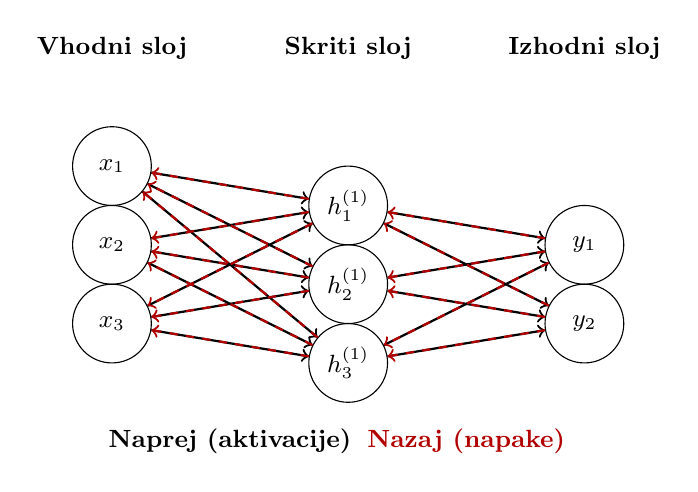
\begin{tikzpicture}[
  neuron/.style={circle, draw, minimum size=1cm},
  arrow/.style={->, thick},
  every node/.style={font=\small}
]

% Layer positions
\foreach \i in {1,...,3}
  \node[neuron] (I\i) at (0, -\i) {$x_{\i}$};

\foreach \i in {1,...,3}
  \node[neuron] (H\i) at (3, -\i - 0.5) {$h^{(1)}_{\i}$};

\foreach \i in {1,...,2}
  \node[neuron] (O\i) at (6, -\i - 1) {$y_{\i}$};

% Forward arrows
\foreach \i in {1,...,3} {
  \foreach \j in {1,...,3}
    \draw[arrow] (I\i) -- (H\j);
}

\foreach \i in {1,...,3} {
  \foreach \j in {1,...,2}
    \draw[arrow] (H\i) -- (O\j);
}

% Backward arrows (dashed)
\foreach \i in {1,...,3} {
  \foreach \j in {1,...,2}
    \draw[->, dashed, red!70!black, thick] (O\j) -- (H\i);
}

\foreach \i in {1,...,3} {
  \foreach \j in {1,...,3}
    \draw[->, dashed, red!70!black, thick] (H\i) -- (I\j);
}

% Labels
\node at (0,0.5) {\textbf{Vhodni sloj}};
\node at (3,0.5) {\textbf{Skriti sloj}};
\node at (6,0.5) {\textbf{Izhodni sloj}};

\node at (1.5,-4.5) {\textcolor{black}{\textbf{Naprej (aktivacije)}}};
\node at (4.5,-4.5) {\textcolor{red!70!black}{\textbf{Nazaj (napake)}}};

\end{tikzpicture}
\caption{Shema propagacije naprej (črne puščice) in nazaj (rdeče prekinjene puščice) v nevronski mreži.}
\label{fig:backprop-shema}
\end{figure}
